 % mainfile: ../../../../master.tex
\label{task:20240401_aosp}
 
\subsection{Complete Lifecycle Hook Execution Flow}

\subsubsection{Android Lifecycle Hooks}

\texttt{onCreate}, \texttt{onStart}, \texttt{onPause}, \texttt{onStop}, \texttt{onResume}, \texttt{onDestroy}\footnote{\url{https://developer.android.com/guide/components/activities/activity-lifecycle}}

\subsubsection{\texttt{onCreate} Hook Ran by \texttt{ActivityThread}}

Look for \texttt{ActivityThread.java} which has \texttt{performLaunchActivity} method which calls \texttt{onCreate}\footnote{\url{https://www.jianshu.com/p/c8e09bc142fa}}

It is called by \texttt{ClientTransactionHandler}'s \texttt{handleLaunchActivity} which is called by \footnote{\url{https://blog.csdn.net/shulianghan/article/details/120263706}}

\subsubsection{What's the difference between \texttt{BIND\_APPLICATION} and \texttt{attachapplication}?}

\path{BIND_APPLICATION} is the message handled by \texttt{ActivityThread} which goes on to call \texttt{attachApplication}.

\subsubsection{What's the difference between Launch Activity vs Start Activity?}

\path{BIND_APPLICATION}\footnote{\url{https://medium.com/android-news/android-application-launch-explained-from-zygote-to-your-activity-oncreate-8a8f036864b}} message is sent to the system server's looper after new process is spawned, to bind the application to the process.

\path{LAUNCH_ACIVITY} is another message after binding the application to launch the main activity of the application \footnote{\url{https://blog.csdn.net/Tenderness4/article/details/83353636}}\footnote{\url{https://juejin.cn/post/7005062882966634526}}\footnote{\url{https://www.zhihu.com/tardis/zm/art/468648584?source_id=1003}}\footnote{\url{https://sleticalboy.github.io/android/2019/04/13/app\%E5\%90\%AF\%E5\%8A\%A8\%E6\%B5\%81\%E7\%A8\%8B\%E5\%88\%86\%E6\%9E\%90-02/}}\footnote{\url{https://sleticalboy.github.io/assets/android/android-app-start.svg}}\footnote{\url{https://dev.to/pyricau/android-vitals-how-adb-measures-app-startup-5n7}}

\subsubsection{How does Zygote call \texttt{ActivityThread}'s \texttt{main}?}

\texttt{ZygoteInit}'s \texttt{main} calls \texttt{ActivityThread}'s constructor which prepares the main looper where all app events are executed\footnote{\url{https://stackoverflow.com/questions/46300145/what-the-matter-between-zygote-and-ui-thread-of-android}}.

\subsubsection{\texttt{runp.sh} for Building, Flashing and Logging Pipeline}
\begin{lstlisting}[language=bash]
adb reboot bootloader

echo "[WEIMINN] Wiping data"

fastboot erase userdata

echo "[WEIMINN] Building AOSP"

cd /media/weiminn/Data/aosp14new

source build/envsetup.sh

lunch aosp_cheetah-userdebug

make

echo "[WEIMINN] Flashing ROM"

fastboot -w flashall

adb wait-for-device

echo "[WEIMINN] Waiting for boot completion"

A=$(adb shell getprop sys.boot_completed | tr -d '\r')

while [ "$A" != "1" ]; do
        echo "[WEIMINN] Waiting for boot completion"
        sleep .5
        A=$(adb shell getprop sys.boot_completed | tr -d '\r')
done

adb root

echo "[WEIMINN] Enabling logging"

adb shell setprop debug.ld.all dlerror,dlopen

rm -f logcat.txt 

echo "[WEIMINN] Logging with Logcat to logcat.txt"

adb logcat >> logcat.txt    
\end{lstlisting}

\subsection{Complete Events Execution Flow}
\subsection{Instrument ART Native Execution Flow}
\subsection{Instrument ART Interpreted Execution Flow}
\subsection{Figure out Debloater Flow} 
\subsection{Sequence Diagram Debloater Flow}
\subsection{Instrument Debloater Flow}
\subsection{Find Links on Permission Manager}
\subsection{Find Links on Package Manager}
\subsection{Explore Package Manager Service Source Codes}
\subsection{Complete Package Manager Loading Flow}
\subsection{Understand Zicheng's Changes to Package Manager}
\subsection{Instrument Package Manager Process}

% 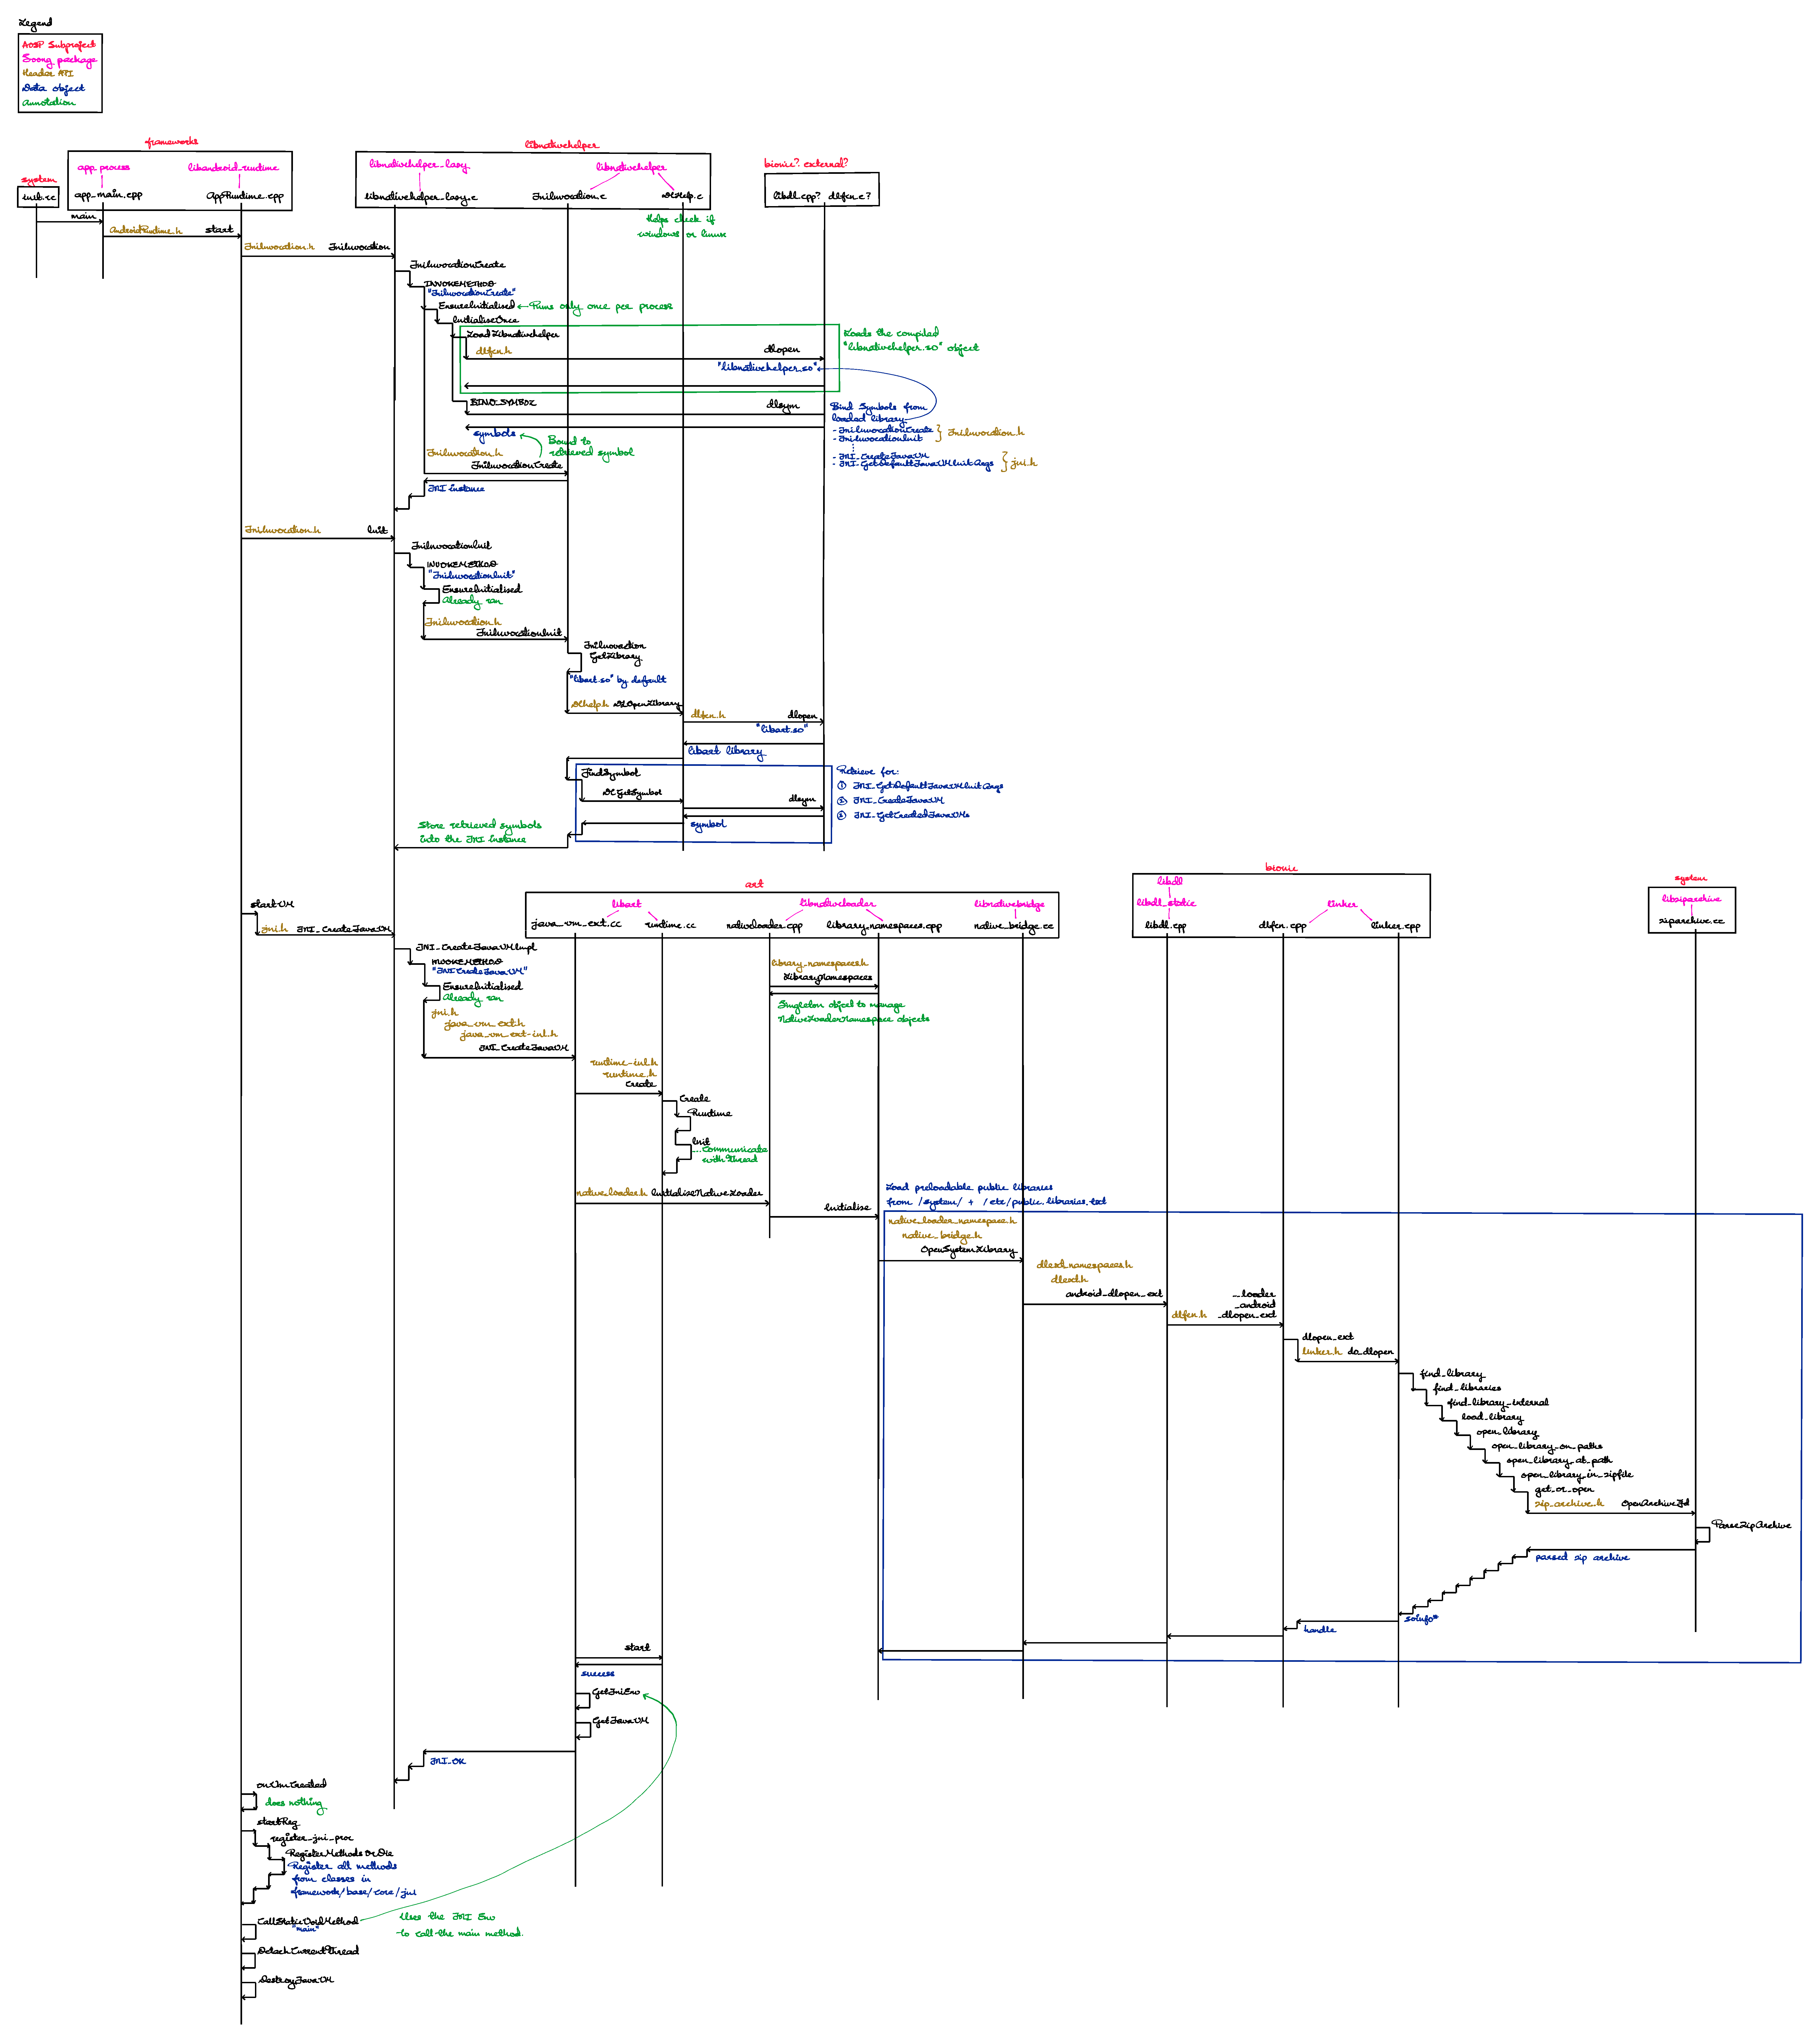
\includepdf[pages=-, scale=.95,pagecommand={}]{entries/2024/01/01/art.pdf}

% \begin{itemize}
% \item \textbf{Domain.} The context of the process that is acting upon something.
% \item \textbf{Type.} The context of the resource on which the process is acting.
% \item \textbf{Class.} The object class of the resource (e.g. \textit{file} or \textit{socket}).
% \item \textbf{Permissions.} The permissions that are allowed given the \textit{domain}, \textit{type} and \textit{class}.
% \end{itemize}

% SELinux rule syntax:


% \subsubsection{Decoding Permission Denial Message}

% Message:
% \begin{lstlisting}
% type=AVC msg=audit(1363289005.532:184): avc:  denied  { read } for  pid=29199 comm="Trace" 
% name="online" dev="sysfs" ino=30 scontext=staff_u:staff_r:googletalk_plugin_t 
% tcontext=system_u:object_r:sysfs_t tclass=file
% \end{lstlisting}

% \begin{longtable}{p{.15\linewidth}p{.15\linewidth}p{.65\linewidth}} 
% \toprule
% Log part & Name & Description \\
% \midrule
% \endhead

% \texttt{type=AVC}
% &Log type
% &Only in the \texttt{audit.log} file; it informs the user what kind of audit log type this is. 
% \\

% \texttt{msg=audit(1363289005.532:184)}
% &Timestamp
% &Timestamp in seconds since epoch, meaning the number of seconds since January 1st, 1970. You can convert this to a more human readable format using date -d @ followed by the number, like so: \texttt{date -d @1363292159.532}.
% \\

% \texttt{avc:}
% &Log type (again)
% &
% \\

% \texttt{ino=30}
% &inode number
% &The inode number of the target file. In this case, since we know it is on the \texttt{sysfs} file system, we can look for this file using: \texttt{find /sys -xdev -inum 30}
% \\

% \texttt{scontent=staff\_u:staff\_r:googletalk\_plugin\_t}
% &Source context
% &The security context of the process (the domain)
% \\

% \texttt{tcontext=system\_u:object\_r:sysfs\_t}
% &Target context
% &The security context of the target resource (in this case the file)
% \\

% \texttt{tclass=file}
% &Target class
% &The class of the target.
% \\

% \midrule
% \caption{Permission Denied Syntax} 
% \label{tab:permissiondeniedsyntax}
% \end{longtable}


% \subsubsection{SELinux Architecture}

% SELinux consists of four main components: object managers (OM), access vector cache (AVC), security server, and security policy as show below:
% \begin{figure}[H]
%     \centering
%     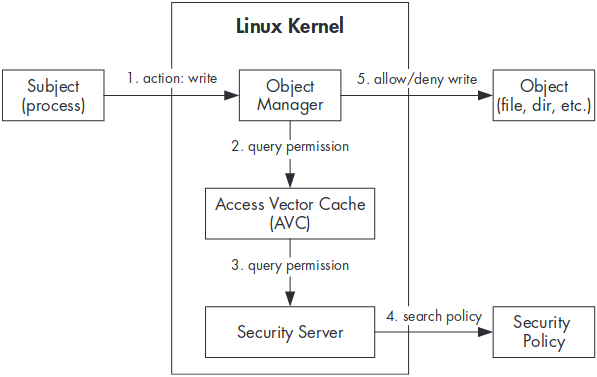
\includegraphics[width=.85\linewidth]{entries/2023/12/10/selinux.png}
%     \caption{SELinux Components}
%     \label{fig:selinux}
% \end{figure}
